\begin{enumerate}[label=\thesection.\arabic*,ref=\thesection.\theenumi]
\numberwithin{equation}{enumi}
\numberwithin{figure}{enumi}
\numberwithin{table}{enumi}
\item Find the angle between two vectors $\overrightarrow{a}$ and $\overrightarrow {b} $ with magnitudes $\sqrt{3}$ and 2 respectively having $\overrightarrow {a}.\overrightarrow {b}=\sqrt{6}$.
	\\
	\solution
		\input{chapters/12/10/3/1/inner.tex}
\item Find the angle between the the vectors $\hat{i}-2\hat{j}+3\hat{k}$ and $3\hat{i}-2\hat{j}+\hat{k}$.
	\\
	\solution
		\input{chapters/12/10/3/2/inner.tex}
\item Find $\abs{\overrightarrow {a}}$ and $\abs{\overrightarrow {b}}$,if ($\overrightarrow {a}+\overrightarrow {b}).(\overrightarrow {a}-\overrightarrow {b})=8$ and $\abs{\overrightarrow {a}}=8\abs{\overrightarrow {b}}$.
	\\
	\solution
		\input{chapters/12/10/3/6/norm.tex}
\item Evaluate the product(3$\overrightarrow {a}-5\overrightarrow {b}).(2\overrightarrow {a}+7\overrightarrow {b}$).
	\\
	\solution
		\input{chapters/12/10/3/7/inner.tex}
\item Find the magnitude of two vectors $\overrightarrow {a}$ and $\overrightarrow {b}$, having the same magnitude and such that the angle between them is $60\degree$ and their scalar product is $\frac{1}{2}$
	\\
	\solution
		\input{chapters/12/10/3/8/inner.tex}
\item Find $\abs{\overrightarrow {x}}$,if for a unit vector $\overrightarrow {a},(\overrightarrow {x}-\overrightarrow {a}).(\overrightarrow {x}+\overrightarrow {a}$)=12.
	\\
		\input{chapters/12/10/3/9/norm.tex}
\item If the vertices A,B,C of a triangle ABC are (1,2,3),(-1,0,0)(0,1,2), respectively , then find  $\angle{ABC}. [\angle{ABC}$ is the angle between the vectors $\overrightarrow{BA}$ and $\overrightarrow{BC}$].
	\\
	\solution
		\input{chapters/12/10/3/15/inner.tex}
    \item Find the direction cosines of a line which makes equal angles with the coordinate
    axes.
		\\
		\solution
		\input{chapters/12/11/1/2/norm.tex}
\item Find a unit vector perpendicular to each of the vector $\overrightarrow{a}+\overrightarrow{b}\text{ and }\overrightarrow{a}-\overrightarrow{b},\text{ where } \overrightarrow{a}=3\hat{i}+2\hat{j}+2\hat{k}\text{ and } \overrightarrow{b}=\hat{i}+2\hat{j}-2\hat{k}$. 
	\\
		\solution
		\input{chapters/12/10/4/2/inner.tex}
\item If a unit vector $\overrightarrow{a}$ makes angles $\dfrac{\pi}{3}\text{ with }\hat{i}, \dfrac{\pi}{4}\text{ with }\hat{j}$ and an acute angle $\theta \text{ with }\hat{k},\text{ then find } \theta$ and hence, the components of $\overrightarrow{a}$.
	\\
		\solution
		\input{chapters/12/10/4/3/norm.tex}
\item Show that the direction cosines of a vector equally inclined to the axes OX, OY and OZ are \textpm $\sbrak{\frac{1}{\sqrt{3}},\frac{1}{\sqrt{3}},\frac{1}{\sqrt{3}}}$.\\
	\solution
		\input{chapters/12/10/5/11/norm.tex}
\item Write down a unit vector in XY-plane, making an angle of 30$^{\circ}$ with the positive direction of x-axis.\\
\item The scalar product of the vector $\hat{i}+\hat{j}+\hat{k}$ with a unit vector along the sum of vectors $2\hat{i}+4\hat{j}-5\hat{k}$ and $\lambda\hat{i}+2\hat{j}+3\hat{k}$ is equal to one. Find the value of $\lambda$.
\item If $\theta$ is the angle between two vectors $\vec{a}$ and $\vec{b}$,then $\vec{a}.\vec{b}\geq0$ only when 
\begin{enumerate}
\item \label{itm:chapters/12/10/5/161} $0<\theta<\frac{\pi}{2}$
\item \label{itm:chapters/12/10/5/162} $0\le\theta\le\frac{\pi}{2}$
\item \label{itm:chapters/12/10/5/163} $0<\theta<\pi$
\item \label{itm:chapters/12/10/5/164} $0\le\theta\le\pi$
\end{enumerate}
	\solution
		\input{chapters/12/10/5/16/inner.tex}
\item Find the slope of the line, which makes an angle of 30 degrees with the positive direction of y-axis measures anticlockwise.
\label{chapters/11/10/1/7}\\
\solution
\input{chapters/11/10/1/7/inner.tex}
\item Find the angle between x-axis and the line joining points (3,-1) and (4,-2).
\label{chapters/11/10/1/10}
\input{chapters/11/10/1/10/matrix.tex}
	\item The slope of a line is double of the slope of another line. If tangent of the angle between them is 1/3, find the slopes of the lines.
\label{chapters/11/10/1/11}
\input{chapters/11/10/1/11/matrix.tex}
\item    Find angle between the lines,$\sqrt{3}x+y=1$ and $x+\sqrt{3}y$=1.
\label{chapters/11/10/3/9}
%\documentclass[12pt]{article}
%\usepackage[cmex10]{amsmath}
%\usepackage{amsthm}
%\usepackage{mathrsfs}
%\usepackage{txfonts}
%\usepackage{stfloats}
%\usepackage{bm}
%\usepackage{cite}
%\usepackage{cases}
%\usepackage{subfig}
%\usepackage{longtable}
%\usepackage{multirow}
%\usepackage{enumitem}
%\usepackage{mathtools}
%\usepackage{steinmetz}
%\usepackage{tikz}
%\usepackage{circuitikz}
%\usepackage{verbatim}
%\usepackage{tfrupee}
%\usepackage[breaklinks=true]{hyperref}
%\usepackage{tkz-euclide} % loads  TikZ and tkz-base
%\providecommand{\brak}[1]{\ensuremath{\left(#1\right)}}
%\usepackage{atbegshi}
%\AtBeginDocument{\AtBeginShipoutNext{\AtBeginShipoutDiscard}}
%\usetikzlibrary{calc,math}
%\usepackage{listings}
%    \usepackage{color}                                            %%
%    \usepackage{array}                                            %%
 %   \usepackage{longtable}                                        %%
  %  \usepackage{calc}                                             %%
   % \usepackage{multirow}                                         %%
    %\usepackage{hhline}                                           %%
    %\usepackage{ifthen}                                           %%
  %optionally (for landscape tables embedded in another document): %%
    %\usepackage{lscape}     
%\usepackage{multicol}
%\usepackage{chngcntr}

%\DeclareMathOperator*{\Res}{Res}
%\renewcommand{\baselinestretch}{2}
%\renewcommand\thesection{\arabic{section}}
%\renewcommand\thesubsection{\thesection.\arabic{subsection}}
%\renewcommand\thesubsubsection{\thesubsection.\arabic{subsubsection}}


% correct bad hyphenation here
%\hyphenation{op-tical net-works semi-conduc-tor}
%\def\inputGnumericTable{}                                 %%

%\lstset{
%language=C,
%frame=single, 
%breaklines=true,
%columns=fullflexible
%}
%\begin{document}
%\newtheorem{theorem}{Theorem}[section]
%\newtheorem{problem}{Problem}
%\newtheorem{proposition}{Proposition}[section]
%\newtheorem{lemma}{Lemma}[section]
%\newtheorem{corollary}[theorem]{Corollary}
%\newtheorem{example}{Example}[section]
%\newtheorem{definition}[problem]{Definition}
%\newcommand{\BEQA}{\begin{eqnarray}}
%\newcommand{\EEQA}{\end{eqnarray}}
%\newcommand{\define}{\stackrel{\triangle}{=}}

%\bibliographystyle{IEEEtran}
%\bibliographystyle{ieeetr}
%\providecommand{\mbf}{\mathbf}
%\providecommand{\pr}[1]{\ensuremath{\Pr\left(#1\right)}}
%\providecommand{\qfunc}[1]{\ensuremath{Q\left(#1\right)}}
%\providecommand{\sbrak}[1]{\ensuremath{{}\left[#1\right]}}
%\providecommand{\lsbrak}[1]{\ensuremath{{}\left[#1\right.}}
%\providecommand{\rsbrak}[1]{\ensuremath{{}\left.#1\right]}}
%\providecommand{\brak}[1]{\ensuremath{\left(#1\right)}}
%\providecommand{\lbrak}[1]{\ensuremath{\left(#1\right.}}
%\providecommand{\rbrak}[1]{\ensuremath{\left.#1\right)}}
%\providecommand{\cbrak}[1]{\ensuremath{\left\{#1\right\}}}
%\providecommand{\lcbrak}[1]{\ensuremath{\left\{#1\right.}}
%\providecommand{\rcbrak}[1]{\ensuremath{\left.#1\right\}}}
%\theoremstyle{remark}
%\newtheorem{rem}{Remark}
%\newcommand{\sgn}{\mathop{\mathrm{sgn}}}
%\providecommand{\res}[1]{\Res\displaylimits_{#1}} 
%\providecommand{\mtx}[1]{\mathbf{#1}}
%\providecommand{\fourier}{\overset{\mathcal{F}}{\rightleftharpoons}}
%\providecommand{\system}{\overset{\mathcal{H}}{\longleftrightarrow}}
	%\newcommand{\solution}[2]{\textbf{Solution:}{#1}}
%\newcommand{\solution}{\noindent \textbf{Solution: }}
%\newcommand{\cosec}{\,\text{cosec}\,}
%\providecommand{\dec}[2]{\ensuremath{\overset{#1}{\underset{#2}{\gtrless}}}}
%\newcommand{\myvec}[1]{\ensuremath{\begin{pmatrix}#1\end{pmatrix}}}
%\newcommand{\mydet}[1]{\ensuremath{\begin{vmatrix}#1\end{vmatrix}}}
%\let\vec\mathbf
%\begin{center}
%\title{\textbf{Straight Lines}}
%\date{\vspace{-5ex}} %Not to print date automatically
%\maketitle
%\end{center}
%\setcounter{page}{1}
%\section*{11$^{th}$ Maths - Chapter 10}
%This is Problem-10 from Exercise 10.4
%\begin{enumerate}
%    \item If three lines whose equations are $y=m_1x+c_1$, $y=m_2x+c_2$ and $y=m_3x+c_3$ are concurrent, then show that $m_1(c_2-c_3)+m_2(c_3-c_1)+m_3(c_1-c_2) = 0.$\\
%    \solution 
    Given lines can be written as \begin{align}
       m_1x-y+c_1=0
    \end{align}
    \begin{align}
        m_2x-y+c_2=0
    \end{align}
    \begin{align}
        m_3x-y+c_3=0
        \label{eq:3}
    \end{align}
    
    
   The above lines can be written in the form of \begin{align}
        \Vec{n}^{\top}\Vec{x} = c
    \end{align}
   Therefore,
		\begin{align}
       \myvec{m_1&-1}\vec{x}=c_1
       \label{eq:5}
   \end{align} 
   \begin{align}
       \myvec{m_2&-1}\vec{x}=c_2
       \label{eq:6}
   \end{align}
   \begin{align}
       \myvec{m_3&-1}\vec{x}=c_3
       \label{eq:7}
   \end{align}
   Solving equations \eqref{eq:5}, \eqref{eq:6}and \eqref{eq:7}
		augumented matrix is
 \begin{align}
    \myvec{m_1&-1&c_1\\m_2&-1&c_2\\m_3&-1&c_3}\\
    \xleftrightarrow{R_2 \leftarrow m_1R_2-m_2R_1}
    \myvec{m_1&-1&c_1\\0&m_2-m_1&m_1c_2-m_2c_1\\m_3&-1&c_3}\\
    \xleftrightarrow{R_3 \leftarrow m_1R_3-m_3R_1}
    \myvec{m_1&-1&c_1\\0&m_2-m_1&m_1c_2-m_2c_1\\0&m_3-m_1&m_1c_3-m_3c_1}\\
    \xleftrightarrow{R_3 \leftarrow R_3\frac{m_2-m_1}{m_3-m_1}-R_2}
        \myvec{m_1&-1&c_1\\0&m_2-m_1&m_1c_2-m_2c_1\\0&0&$\brak{m_1c_3-m_3c_1}$$\brak{\frac{m_2-m_1}{m_3-m_1}}$-$\brak{m_1c_2-m_2c_1}$}
\end{align}
Now, for lines to be concurrent, then the third row should be equal to zero. \\

Therefore,
\begin{align}
\brak{m_1c_3-m_3c_1}\brak{\frac{m_2-m_1}{m_3-m_1}}-\brak{m_1c_2-m_2c_1}=0\\
\frac{\brak{m_1c_3-m_3c_1}\brak{m_2-m_1}-\brak{m_1c_2-m_2c_1}\brak{m_3-m_1}}{m_3-m_1}=0\\
\brak{m_1c_3-m_3c_1}\brak{m_2-m_1}-\brak{m_1c_2-m_2c_1}\brak{m_3-m_1}=0\\
m_2c_3-m_1c_3+m_3c_1-m_3c_2+m_1c_2-m_2c_1=0\\
m_1\brak{c_2-c_3}+m_2\brak{c_3-c_1}+m_3\brak{c_1-c_2} = 0
\end{align}
           Hence proved
%\begin{figure}[h]
 %   \centering
  %  \includegraphics[width=\columnwidth]{concurrent-1.png}
   % \caption{Straight Lines}
    %\label{fig:concurrent-1.png}
%\end{figure}
%\end{enumerate}
%\end{document}

\item Find the equation of the lines through the point (3, 2) which make an angle of 45\degree  with the line $x – 2y$ = 3.
\label{chapters/11/10/4/11}\\
\solution
%\documentclass{article}
%\documentclass[10pt,a4paper]{report}
%\usepackage{amsmath}
%\usepackage{amssymb}
%\usepackage{gensymb}
%\usepackage{amsfonts}
%\usepackage{setspace}
%\usepackage{tasks}
%\usepackage{graphicx}
%\usepackage{float}
%\usepackage{listings}
%\newcommand{\myvec}[1]{\ensuremath{\begin{pmatrix}#1\end{pmatrix}}}
%\let\vec\mathbf
%\providecommand{\sbrak}[1]{\ensuremath{{}\left[#1\right]}}
%\providecommand{\lsbrak}[1]{\ensuremath{{}\left[#1\right.}}
%\providecommand{\rsbrak}[1]{\ensuremath{{}\left.#1\right]}}
%\providecommand{\brak}[1]{\ensuremath{\left(#1\right)}}
%\providecommand{\lbrak}[1]{\ensuremath{\left(#1\right.}}
%\providecommand{\rbrak}[1]{\ensuremath{\left.#1\right)}}
%\providecommand{\cbrak}[1]{\ensuremath{\left\{#1\right\}}}
%\providecommand{\lcbrak}[1]{\ensuremath{\left\{#1\right.}}
%\providecommand{\rcbrak}[1]{\ensuremath{\left.#1\right\}}}
%\providecommand{\norm}[1]{\left\lVert#1\right\rVert}
%\providecommand{\abs}[1]{\left\vert#1\right\vert}
%\let\vec\mathbf
%\newcommand{\norm}[1]{\lVert#1\rVert}
%\renewcommand{\vec}[1]{\textbf{#1}}
%\begin{document}
%\onehalfspacing
%\begin{center}
%	\section*{\textbf{Class 11}}
%	\subsection*{Chapter 10 - STRAIGHT LINES}
%\end{center}
%The following problem is question 11 from exercise 10.4
%\begin{enumerate}
 %   \item Find the equation of the lines through the point (3, 2) which make an angle of 45\degree  with the line x – 2y = 3.
%\end{enumerate}
%\textbf{Solution:}\\
The given line parameters are
\begin{align}
   \vec{n}=\myvec{1\\-2},c=-5\\
	\vec{P}=\myvec{3\\2}
\end{align}
yielding
\begin{align}
\vec{m}_1=\myvec{2\\1}\\
\vec{m}_2=\myvec{1\\m}
\end{align}
where  $m$ is defined to be the slope of the line. If the angle between the lines be $\theta$,

\begin{align}
\cos \theta = \frac{\vec{m}_1^\top \vec{m}_2}{\norm{\vec{m}_1}\norm{\vec{m}_2}}\\
	\text{given, } \theta = 45\degree\\
\implies \cos45\degree =  \frac{\vec{m}_1^\top \vec{m}_2}{\norm{\vec{m}_1}\norm{\vec{m}_2}}\\
\implies \frac{1}{\sqrt{2}} = \frac{\myvec{2 & 1} \myvec{1\\m}}{\norm{\myvec{2\\1}}\norm{\myvec{1\\m}}}
\end{align}
\begin{align}
\implies \frac{1}{\sqrt{2}}=\frac{2+m}{\sqrt{2^2 + 1}\sqrt{m^2 + 1}}\\
\implies \frac{1}{2}=\frac{m^2 + 4m +4}{5m^2 +5}\\
\text{or, } 3m^2 - 8m -3 = 0
\end{align}
yielding
\begin{align}
m= - \frac{1}{3}, 3
\end{align} 
when m=3,the equation of line passing through $\vec{P}$  is then obtained as
\begin{align}
\vec{n}^{\top} ({\vec{x}-\vec{P}}) = 0\\
\text{where,}{\vec{n}}=\myvec{m\\-1} \\
{\vec{n}}=\myvec{3\\-1} \\
\implies 
	\myvec{3&-1}\cbrak{\vec{x}-\myvec{3\\2}}&=0\\
	&=7 \\
 \implies 	\myvec{3 & -1}\vec{x} &= 7
\end{align}
And, when $m=-\frac{1}{3}$,the equation of the line passing through $\vec{P}$  and having a slope of $-\frac{1}{3}$is
\begin{align}
\vec{n}^{\top} ({\vec{x}-\vec{P}}) = 0\\
{\vec{n}}=\myvec{-\frac{1}{3}\\-1} \\
\implies {\vec{n}}=\myvec{1\\3} \\
\implies 
	\myvec{1&3}\cbrak{\vec{x}-\myvec{3\\2}}&=0\\
	&=9 \\
		\implies 	\myvec{1 & 3}\vec{x} &= 9
\end{align}
Therefore,the equations of the lines are 
\begin{align}
	\myvec{3 & -1}\vec{x} = 7  \text{ and }   \myvec{1 & 3}\vec{x} = 9 .
\end{align}
%\begin{figure}[H]
%\centering
%\includegraphics[width=\columnwidth]{figs/strline.jpg}
%\caption{STRAIGHT LINES}
%\label{fig:strline.jpg}
%\end{figure}




%\end{document}

\begin{figure}[H]
\centering
\includegraphics[width=\columnwidth]{chapters/11/10/4/11/figs/strline.jpg}
\caption{STRAIGHT LINES}
\label{fig:chapters/11/10/4/11/figs/strline.jpg}
\end{figure}
\item\textbf{}The scalar product of the vector $\hat{i}+\hat{j}+\hat{k}$ with a unit vector along the sum of vectors $2\hat{i}+4\hat{j}-5\hat{k}$ and $\lambda\hat{i}+2\hat{j}+3\hat{k}$ is equal to one, Find the value of $\lambda$.
\\\\
\textbf{Generalized Construction:}\\
We now that \\
\begin{align}
   &\implies \vec{A}^\top = \frac{\brak{\vec{B}+\vec{C}}}{\norm{\vec{B}+\vec{C}}}\\
       &\implies \vec{A}^\top \brak{\vec{B}+\vec{C}}=\norm{\vec{B}+\vec{C}} \label{eq:Eqat2}\\
       &\implies \vec{C}=\lambda\vec{e}_1+\vec{D}\label{eq:EQT-C}
    \end{align}
    were,
    \begin{align}
       &\implies \norm{\vec{B}+\vec{C}}= \sqrt{\brak{\vec{B}+\vec{C}}^\top\brak{\vec{B}+\vec{C}}}
    \end{align}
From the Equation\eqref{eq:Eqat2},We can do
\begin{align}
   &\implies \vec{A}^\top \brak{\vec{B}+\vec{C}}=\sqrt{\brak{\vec{B}+\vec{C}}^\top\brak{\vec{B}+\vec{C}}}\\
&\implies \vec{A}^\top \brak{\vec{B}+\vec{C}}=\sqrt{\norm{\vec{B}}^2+2\sbrak{\vec{B}^{\top}\vec{C}}+\norm{\vec{C}}^2}\\
&\implies \vec{A}^\top \brak{\vec{B}+\vec{C}}=\sqrt{{\vec{B}^{\top}\vec{B}}+2\sbrak{\vec{B}^{\top}\vec{C}}+{\vec{C}^\top\vec{C}}}\label{eq:Eqt6}
\end{align}
Substitute the $\vec{C}$ Value in the Equation\eqref{eq:Eqt6},We get
\begin{align}
&\implies\vec{A}^{\top}\brak{\vec{B}+\lambda\vec{e}_1+\vec{D}}=\sqrt{\vec{B}^{\top}\vec{B}+2\vec{B}^{\top}\brak{\lambda\vec{e}_1+\vec{D}}+\brak{\lambda\vec{e}_1+\vec{D}}^{\top}\brak{\lambda\vec{e}_1+\vec{D}}}
\end{align}
S.O.B.S,we get
\begin{align}
&\implies\brak{\vec{A}^{\top}\brak{\vec{B}+\lambda\vec{e}_1+\vec{D}}}^{2}=\vec{B}^{\top}\vec{B}+2\vec{B}^{\top}\brak{\lambda\vec{e}_1+\vec{D}}+\brak{\brak{\lambda\vec{e}_1+\vec{D}}^{\top}\brak{\lambda\vec{e}_1+\vec{D}}} \\
&\implies\brak{\vec{A}^{\top}\lambda\vec{e}_1}^{2}+\brak{\vec{A}^{\top}\vec{B}+\vec{D}}^{2}+2\brak{\vec{A}^{\top}\lambda\vec{e}_1}\brak{\vec{A}^{\top}\brak{\vec{B}+\vec{D}}}=\vec{B}^{\top}\vec{B}+2\vec{B}^{\top}\brak{\lambda\vec{e}_1+\vec{D}}+\lambda^{2}+2\lambda\vec{e}_1^{\top}\vec{D}+\vec{D}^{\top}\vec{D}\\
&\implies\brak{\lambda^{2}}+\brak{\vec{A}^{\top}\brak{\vec{B}+\vec{D}}}^{2}+2\brak{\vec{A}^{\top}\lambda\vec{e}_1}\brak{\vec{A}^{\top}\brak{\vec{B}+\vec{D}}}=\vec{B}^{\top}\vec{B}+2\lambda\brak{\vec{B}^{\top}\vec{e}_1+\vec{e}_1^{\top}\vec{D}}+\vec{D}^{\top}\vec{D}+\lambda^{2}\\
&\implies2\lambda\sbrak{\vec{A}^\top\vec{e}_1\vec{A}^\top\brak{\vec{B}+\vec{D}}-\brak{\vec{B}^{\top}\vec{e}_1+\vec{e}_1^{\top}\vec{D}}}=\vec{B}^{\top}\vec{B}+2\lambda\brak{\vec{B}^{\top}\vec{e}_1+\vec{e}_1^{\top}\vec{D}}+\vec{D}^{\top}\vec{D}-\brak{\vec{A}^{\top}\brak{\vec{B}+\vec{D}}}^{2}\\
&\implies2\lambda=\frac{\vec{B}^{\top}\vec{B}+2\vec{B}^{\top}\vec{D}+\vec{D}^{\top}\vec{D}-\brak{\vec{A}^{\top}\brak{\vec{B}+\vec{D}}}^{2}}{\sbrak{\vec{A}^\top\vec{e}_1\vec{A}^\top\brak{\vec{B}+\vec{D}}-\brak{\vec{B}^{\top}\vec{e}_1+\vec{e}_1^{\top}\vec{D}}}}\\
&\implies\lambda=\frac{\vec{B}^{\top}\vec{B}+2\vec{B}^{\top}\vec{D}+\vec{D}^{\top}\vec{D}-\brak{\vec{A}^{\top}\brak{\vec{B}+\vec{D}}}^{2}}{2\sbrak{\vec{A}^\top\vec{e}_1\vec{A}^\top\brak{\vec{B}+\vec{D}}-\brak{\vec{B}^{\top}\vec{e}_1+\vec{e}_1^{\top}\vec{D}}}} \label{eq:EWQ77}
\end{align}
Substitute the Given Data in Equation\eqref{eq:EWQ77},
\begin{align*}
\vec{A}=\myvec{1\\1\\1};\vec{B}=\myvec{2\\4\\-5};\vec{C}=\myvec{\lambda\\2\\3}
\end{align*}
we get,
\begin{align}   
&\implies\lambda=\frac{45-14+13-36}{2\brak{1\brak{6}-2}}\\
&\implies\lambda=\frac{44-36}{8}\\
&\impliedby\lambda=\frac{8}{8}\\
 &\implies \lambda = 1
 \begin{enumerate}
 
    \item \textbf{Question(MATH-12.10.5.17):}
       Let $\vec{a}$ and $\vec{b}$ be two unit vectors and $\theta$ is the angle between them. Then $\vec{a}+\vec{b}$ is a unit vector.
    
 \begin{enumerate}[label=(\Alph*)]                     
 \item $\theta$=$\frac{\pi}{4}$
 \item $\theta$=$\frac{\pi}{3}$
  \item $\theta$=$\frac{\pi}{2}$
   \item $\theta$=$\frac{2\pi}{3}$
   \end{enumerate}
		 \textbf{solution:}

Given,
\begin{align}
	\norm{\vec{a}} &= \norm{\vec{b}}=1 
 \label{eq:eq1},\\
	\norm{\vec{a}+\vec{b}}&=1
 \label{eq:eq0}
 \end{align}
Squaring on both sides of \eqref{eq:eq0}, we get
\begin{align}
	\norm{\vec{a}+\vec{b}}^2 &=1^2
\\	
	\implies \norm{\vec{a}}^2 + \norm{\vec{b}}^2 + 2\vec{a}^{\top}\vec{b} &= 1
 \label{eq:eq2}
\end{align}

Substituting \eqref{eq:eq1} in \eqref{eq:eq2}, we get

\begin{align}
	\implies 1+1+2(\norm{\vec{a}}\norm{\vec{b}}\cos{\theta}) &=1\\
	\implies 2+2(\norm{\vec{a}}\norm{\vec{b}}\cos{\theta}) &=1\\
	\implies 2(\norm{\vec{a}}\norm{\vec{b}}\cos{\theta}) &=-1\\
	\implies (\norm{\vec{a}}\norm{\vec{b}}\cos{\theta}) &=\frac{-1}{2}
 \label{eq:eq3}
\end{align}
Substituting \eqref{eq:eq1} in \eqref{eq:eq3}, we get
\begin{align}
	\implies \cos{\theta} &=\frac{-1}{2}
	\\
	\implies \theta &=\frac{2\pi}{3}
\end{align}

Let, \begin{align}
	\vec{a} &= \myvec{\cos \theta_1 \\ \sin \theta_1}\\
	\vec{b} &= \myvec{\cos \theta_2 \\ \sin \theta_2}
\end{align}
Matrix multiplication of $\vec{a}.\vec{b}$ is:
\begin{align}
	\vec{a}^{\top}\vec {b}= \cos \brak{\theta_1 -\theta_2} &= \frac{-1}{2}\\
	\theta_1 - \theta_2& =\cos^{-1} \brak{\frac{-1}{2}}\\
	\theta_1 - \theta_2 &= \frac{2\pi}{3}\\
	\theta_1 &= \theta_2 +\frac{2\pi}{3}
\end{align}
  \begin{figure}[H]
	  \centering        
	  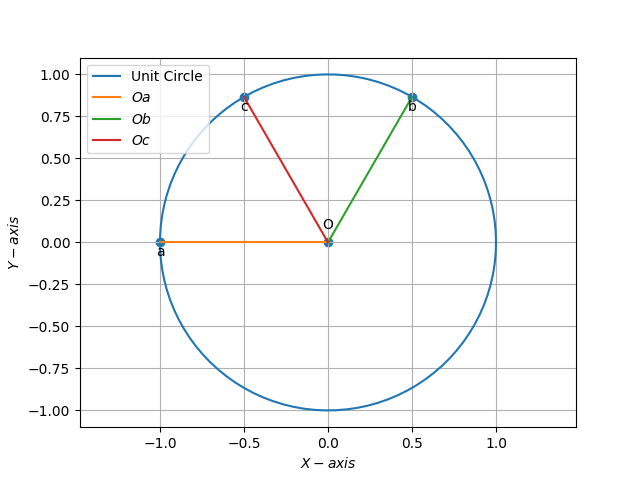
\includegraphics[width=\columnwidth]{/home/himabindu/figures/figg.png}
	  \caption{}       
	  \label{fig:python generated plot}
  \end{figure}
\end{align}
\end{enumerate}
